\documentclass{article}
\usepackage[a4paper, margin=0.7in, top=1in]{geometry}
\usepackage[table]{xcolor}
\usepackage[mathscr]{euscript}
\usepackage[ruled,vlined]{algorithm2e}
\usepackage{pgfplotstable}
\usepackage{amsmath}
\usepackage{amsfonts}
\usepackage{multicol}
\pgfplotsset{compat=1.17}

\begin{document}
\title{A k-flip local search algorithm for SAT and MAX SAT}
\author{Chris Patuzzo}
\maketitle

\abstract
Local search can be applied to SAT by determining whether it is possible to
increase the number of satisfied clauses for a given truth assignment by
flipping at most $k$ variables. However, for a problem instance with $v$
variables, the search space is of order $v^k$. A naive approach that enumerates
every combination is impractical for all but the smallest of problems. This
paper outlines a hybrid approach that plays to the strength of modern SAT
solvers to search this space more efficiently. We describe an encoding of SAT
to a related problem –\linebreak k-Flip MAX SAT – and show how, through repeated
application, it can be used to solve SAT and MAX SAT problems. Finally, we test
the algorithm on a benchmark set with different values of $k$ to see how it
performs.

\section{Introduction}

Modern SAT solvers are able to cope with formulas that contain many hundreds or
thousands of variables. In doing so, they employ a variety of techniques. One
such category of techniques is that of local search. The basic idea is that,
for some notion of locality and for as long as possible, a SAT solver can
transition from one candidate solution to another with the intention of
improving its quality. A typical measure of quality is the number of clauses
satisfied by the candidate solution – a truth assignment to variables in the
formula.

One such notion of locality is the number of variables that have been ‘flipped’
from one canditate solution to another, i.e. the number of truth assignments
that differ. We say that two truth assignments are ‘k-flip neighbors’ if they
differ in the values of at most $k$ variables[?]. The question of whether a
“better” candidate solution exists under this notion of locality can be
formalised into a decision problem:\\

k-\textsc{flip max sat}

Question: Is there a k-flip neighbor for truth assignment $A$ that satisfies
more clauses in formula $F$ than $A$? \\

\noindent For a formula that contains $v$ variables, this decision problem is
of order $\mathcal{O}(v^k)$ which grows very quickly. However, in practice we
may be able to decide this efficiently using a SAT solver. Whatsmore, when used
as the basis of a local search algorithm, the k-\textsc{flip max sat} decision
problem is decided multiple times.

A fairly recent development in SAT solving has been the introduction of the
IPASIR interface. This allows a given formula to be solved multiple times under
different assumptions. In doing so, the SAT solver is able to preserve much of
its ‘knowledge’ about the formula, for example, learned clauses from the CDCL
process. If the k-\textsc{flip max sat} problem is to be used as the basis for
a local search algorithm, it seems likely that the algorithm's performance
would benefit from this incremental approach.

Perhaps a more interesting line of investigation is to test the efficacy of
local search in deciding SAT, through repeated application of the
k-\textsc{flip max sat} decision problem. To what extent can a candidate
solution be improved through this process before no k-flip neighbor exists that
satisfies more clauses? Therefore, in this paper we investigate the following
questions: \\

- How can we encode the SAT problem into an instance of the k-\textsc{flip max sat} problem?

- How can we use this encoding as the basis of an incremental local search algorithm?

- How long does our incremental local search algorithm take as we vary $k$?

- How effective is local search (using k-flips) at solving SAT (and MAX SAT) problems? \\

\noindent The last two questions are problem-dependent so it's difficult to
make general claims about them. We limit the scope of our investigation to a
benchmark set of uniform random 3-SAT instances.

\break

\section{The encoding}

At a high level, the encoding takes some SAT formula $F$ and parameter $k$ and
transforms it into a new SAT formula $F'$ that is satisfiable if and only if
$F$ is satisfiable subject to two numerical constraints:

\begin{enumerate}
  \item The first numerical constraint enforces the ‘k-flips’ requirement. A
    set of variables $A$ is introduced that represents some truth assignment
    for $F$. A corresponding set of variables $A'$ is added that is allowed to
    differ by at most $k$ truth values from $A$. Intuitively, this delta is the
    subset of variables that has been ‘flipped’. We use a counter circuit and a
    less-than comparator to enforce this constraint.

  \item The second numerical constraint limits the number of unsatisfied
    clauses in $F$ subject to the set of truth values $A'$. For each clause in
    $F$, we introduce a variable whose intended meaning is that its related
    clause has not been satisfied by $A'$. Collectively, we call this set $U$.
    We once again use a counter circuit and less-than comparator to enforce
    that the number of true literals in $U$ is less than some value.
\end{enumerate}

\noindent Our encoding has the advantage of separating its numerical
constraints from their threshold values. The latter can either by specified by
appending unit clauses to $F'$ or through assumptions as part of the IPASIR
interface.

\subsection{Flipped variables}

Let $\#v$ be the number of variables in $F$. Add a clause to $F'$ that is
satisfied if either $A_i$ and $A'_i$ have the same truth value or $Fl_i$ is
true. Formula \ref{flipped2} is equivalent to Formula \ref{flipped1} but is
rewritten in conjunctive normal form.

\begin{equation}
  \label{flipped1}
  \bigwedge\limits_{i=1}^{\#v} A_i \to A'_i \lor Fl_i
\end{equation}\break

\begin{equation}
  \label{flipped2}
  \bigwedge\limits_{i=1}^{\#v} \neg{A_i} \lor A'_i \lor Fl_i
\end{equation}\break

\noindent The intended meaning of $Fl_i$ is that variable $i$ in $F$ has been
flipped from some pre-assigned truth value $A_i$ to a new value $A'_i$. However,
we do not add clauses that preclude $Fl_i$ from being true when $A_i$ and $A'_i$
are assigned the same value. In practice, it is never advantageous for a SAT
solver to do so due to the numeric constraints.

\subsection{Unsatisfied clauses}

Let $\#c$ be the number of clauses in $F$. Add a clause to $F'$ that is
satisfied if either clause $i$ in $F$ is satisfied or $U_i$ is true. Again, we
do not preclude $U_i$ from being true when clause $i$ is already satisfied.

\begin{equation}
  \label{unsat}
  \bigwedge\limits_{i=1}^{\#c} Clause_i \lor U_i
\end{equation}\break

\subsection{Parallel counter}

We encode two separate parallel counter circuits into $F'$. The first operates
on $Fl$ and the second on $U$. Since the method of encoding is the same, we
discuss it in general terms for a set $\mathscr{S}$. The objective of the
encoding is to introduce a set of variables $\mathscr{C}$ of size $\lceil
log_2(\mathscr{S}) \rceil$ such that the formula $F'$ is satisfiable if and
only if $\mathscr{C}$ is assigned truth values representing a binary number
equal to the count of true literals in $\mathscr{S}$.

The encoding works by first applying a half-adder gate to consecutive,
non-overlapping pairs of variables $a, b \in \mathscr{S}$. We use a propagation
complete encoding (Formula \ref{halfadder}) which can be derived from the
propagation complete encoding of a full-adder (Formula \ref{fulladder}) by
setting $carry_{in}$ to \textbf{false} and simplifying.

\begin{equation}
  \label{halfadder}
  \begin{split}
    a \lor \neg{b} \lor sum \\
    \neg{a} \lor \neg{b} \lor \neg{sum} \\
    \neg{a} \lor carry_{out} \lor sum \\
    a \lor \neg{carry_{out}} \lor \neg{sum} \\
    b \lor \neg{carry_{out}} \\
    a \lor b \lor \neg{sum} \\
  \end{split}
\end{equation}\break

\noindent The encoding then proceeds recursively. It subdivides the auxiliary
variables produced by the half-adders until either one or two pairs of variables
remain. If two pairs remain, a full-adder (Formula \ref{fulladder}) sums the
result. Afterwards a ripple-carry adder is used to recombine these sums. A
ripple-carry also makes use of multiple full-adders. Its description is omitted
here because it is encoded in a conventional way.

\begin{equation}
  \label{fulladder}
  \begin{split}
    a \lor \neg{b} \lor carry_{in} \lor sum \\
    a \lor b \lor \neg{carry_{in}} \lor sum \\
    \neg{a} \lor \neg{b} \lor carry_{in} \lor \neg{sum} \\
    \neg{a} \lor b \lor \neg{carry_{in}} \lor \neg{sum} \\
    \neg{a} \lor carry_{out} \lor sum \\
    a \lor \neg{carry_{out}}\lor \neg{sum} \\
    \neg{b} \lor \neg{carry_{in}} \lor carry_{out} \\
    b \lor carry_{in} \lor \neg{carry_{out}} \\
    \neg{a} \lor \neg{b} \lor \neg{carry_{in}} \lor sum \\
    a \lor b \lor carry_{in} \lor \neg{sum} \\
  \end{split}
\end{equation}\break

\noindent In general, when two N-bit binary numbers are summed, this can result
in an (N+1)-bit binary number. However, since we know the sum will not exceed
$\vert \mathscr{S} \vert$, there is no need to introduce redundant auxiliary
variables that would always be false. This is a small optimisation that also
helps the SAT solver reject assignments that would inevitably lead to conflict
when the less-than clauses are considered.

\subsection{Less-than comparator}

The less-than comparator makes use of three logical operators: \textsc{and},
\textsc{or} and \textsc{eq}. We use the Tseitin encodings of these gates as
shown in Formulas \ref{and}, \ref{or} and \ref{eq} respectively.

\begin{multicols}{3}
  \begin{equation}
    \label{and}
    \begin{split}
      \neg{a} \lor \neg{b} \lor out \\
      a \lor \neg{out} \\
      b \lor \neg{out} \\
    \end{split}
  \end{equation}\break

  \begin{equation}
    \label{or}
    \begin{split}
      a \lor b \lor \neg{out} \\
      \neg{a} \lor out \\
      \neg{b} \lor out \\
    \end{split}
  \end{equation}\break

  \begin{equation}
    \label{eq}
    \begin{split}
      \neg{a} \lor \neg{b} \lor out \\
      a \lor b \lor out \\
      a \lor \neg{b} \lor \neg{out} \\
      \neg{a} \lor b \lor \neg{out} \\
    \end{split}
  \end{equation}\break
\end{multicols}

\noindent First, we define a new operator that takes two variables and sets
$out$ to true when $a$ is strictly less than $b$.

\begin{equation}
  \textsc{lt}(a, b) = \textsc{and}(\neg{a}, b)
\end{equation}\break

\noindent We then define a recursive operator for two sets of variables $A$,
$B$ and $i \in \mathbb{Z}^*$.

\begin{equation}
  \textsc{lt}^*(A, B, i) = \begin{cases}
    \textsc{lt}(A_i, B_i) & i = 0 \\
    \textsc{or}(\textsc{lt}(A_i, B_i), \textsc{and}(\textsc{eq}(A_i, B_i), \textsc{lt}^*(A, B, i - 1))) & i > 0
  \end{cases}
\end{equation}\break

\noindent The $\textsc{lt}^*$ operator tests whether variable $A_i$ is strictly
less than $B_i$. If it is, the output of the operator is true. Otherwise, if
they are equal, it recursively tests the $i - 1$th bit until $i$ reaches $0$. We
use the convention that index $0$ is the least-significant bit and index $\vert
A \vert - 1$ is the most-significant bit of a binary number.

Finally, we encode the constraint that the binary number represented by
$\mathscr{C}$ is less than some threshold value $\mathscr{T}$ (such that  $\vert
\mathscr{T} \vert = \vert \mathscr{C} \vert$) by conjuncting clauses generated
by the $\textsc{lt}^*$ operator.

\begin{equation}
  \bigwedge \textsc{lt}^*(\mathscr{C}, \mathscr{T}, \vert \mathscr{T} \vert - 1)
\end{equation}

\break

\section{The algorithm}

We make use of our encoding in a local search algorithm that tries to improve
the number of satisfied clauses for some formula $F$. We start with a randomly
generated truth assignment $A$ and make repeated calls to an IPASIR-compatible
SAT solver to improve the candidate solution's quality on each iteration. \\

\begin{algorithm}[H]
\SetAlgoLined
\DontPrintSemicolon

  \KwIn{A CNF formula F}
  \KwIn{An integer k}
  \KwOut{Whether all clauses in F have been satisfied}
  \;

  S $\gets$ initialize\_solver()\;
  F' $\gets$ encode(F, k)\tcp*{Also encodes the k threshold value as unit clauses.}\;
  v $\gets$ num\_vars(F)\;
  A $\gets$ pick\_random(v, \{true, false\})\tcp*{We start with a random truth assignment for F.}\;
  S.assume(A)\;
  \;

  \While{S.solution\_exists()}{
    T $\gets$ S.solution()\tcp*{These assignments includes all auxiliary variables.}\;
    A' $\gets$ decode\_new\_assignments(T)\tcp*{These are the assignments we actually care about.}
    S.assume(A')\tcp*{The previous assumptions are dropped automatically.}
    \;
    u $\gets$ decode\_unsat\_clause\_count(T)\;
    U $\gets$ encode\_unsat\_threshold(u)\tcp*{On the next iteration there must be fewer unsat clauses.}
    S.assume(U)\;
    \;
    print(“k-flips solution: ”, A')\;
    print(“clauses remaining: ”, u)\;
    if u == 0 \{ break \}\tcp*{Break if all clauses are satisfied.}
 }
 \;
  \eIf{u == 0}{
    print(“fully satisfied all clauses for k=”, k)\;
    return true
  } {
    print(“stuck at ”, u, “, no more k-flips exist”)\;
    return false
  }
 \caption{Our incremental k-flips local search algorithm}
\end{algorithm} \vspace{5mm}

\noindent While a solution exists, it means the SAT solver was able to find a
k-flip improvement over $A$ which we decode as $A'$. We assume this new set of
truth assignments for the next iteration of the algorithm. Additionally, we set
a new threshold value for the number of unsatisfied clauses to ensure the
solution quality improves each time. We do this by assuming a value equal to
the current number of unsatisfied clauses.

The algorithm terminates when either no solution exists, i.e. when no k-flip
improvement exists, or when all clauses in $F$ have been satisfied. We return
true or false to indicate this. We also print each k-flip solution and the
number of unsatisfied clauses which we use for our analysis. Since our algorithm
is solving the unweighted MAX SAT problem, the real implementation outputs in a
format compliant with the SAT Competition[?].

One small caveat is that the output of our program may incorrectly report an
inflated number of unsatisfied clauses. This is due to our encoding in Section
2.2 which does not preclude $U_i$ from being true when clause $i$ is already
satisfied. In practice, the correct count can always be recovered by testing
the candidate solution on $F$ and tighter bounds could be placed on $U$ in each
iteration. Since this optimisation does not affect the overall correctness of
our algorithm, we omit it here for brevity.

\break

\section{Empirical results}

We test our algorithm on a SATLIB benchmark set of 1000 uniform random 3-SAT
instances. Each containing 100 variables and 430 clauses. For each formula, we
measure how long it takes the algorithm to run to completion for values of $k$
up to 20. Since our algorithm uses random initialization, we repeat the test
five times for each formula. Figure 1 plots the median completion time in
seconds across all runs.

We also measure k=0 to establish a baseline for the overhead of encoding the
problem, calling the SAT solver, etc. In aggregate, we ran our algorithm 105,000
times which took 80 CPU hours on an Intel i7-7660U. We used Cadical 1.3.1 as the
incremental solver and called it 6,000,000 times. \\

\begin{figure}[htp]
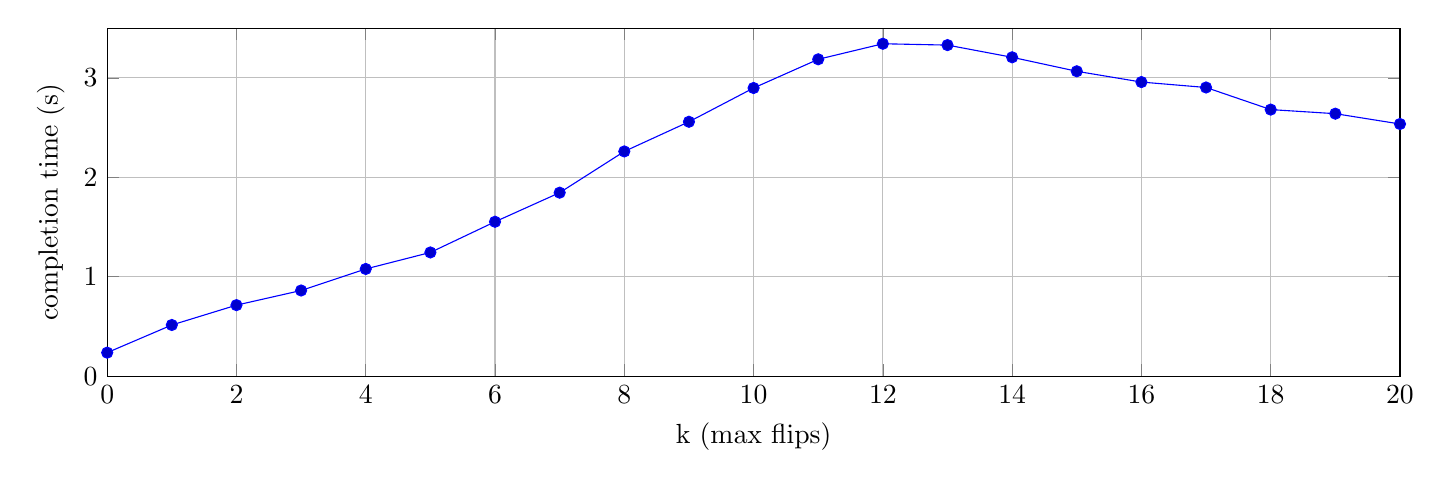
\begin{tikzpicture}
  \begin{axis}[
    height=6cm,
    width=18cm,
    grid=major,
    xlabel=k (max flips),
    ylabel=completion time (s),
    xmin=0, xmax=20,
    ymin=0, ymax=3.5,
  ]

  \addplot coordinates {
    (0, 0.23613068)
    (1, 0.514448288)
    (2, 0.714127463)
    (3, 0.861471642)
    (4, 1.078018418)
    (5, 1.244326101)
    (6, 1.552850239)
    (7, 1.845506096)
    (8, 2.260462076)
    (9, 2.558738066)
    (10, 2.898591395)
    (11, 3.187362312)
    (12, 3.343761958)
    (13, 3.330205619)
    (14, 3.20757239)
    (15, 3.066834229)
    (16, 2.958273301)
    (17, 2.903730373)
    (18, 2.681392024)
    (19, 2.640207394)
    (20, 2.536441681)
  };
  \end{axis}
\end{tikzpicture}
\caption{The median completion time of our algorithm for different values of k}
\end{figure}

\noindent Clearly, the completion time is not growing exponentially in $k$ for
this benchmark set. We speculate the decline in completion time after $k=12$ is
due to the ‘k-flips’ constraint becoming insignificant with larger $k$, to the
extent the SAT solver is infrequently running into conflict with those
constraints. It's likely this benchmark set is too easy for the SAT solver and
an interesting line of investigation would be to evaluate the algorithm on a
more challenging set such as the SAT Competition instances.

We also test the efficacy of k-flip local search on this benchmark
set, irrespective of our algorithm. We measure how many clauses are satisfied
when no k-flip improvement exists and the algorithm terminates. Table 1 plots
a heatmap that counts the number of runs that could be improved no further past
some number of clauses, up to a maximum of 430 which is when all clauses have
been satisfied for problems in this benchmark set. \\

\pgfplotstableset{
  every head row/.style={after row=\hline},
  every first column/.style={column type/.add={}{|}},
  columns/x/.style={column name={}, postproc cell content/.code={}},
  color cells/.style={
    postproc cell content/.code={%
      \pgfkeysalso{@cell content=\rule{0cm}{2.4ex}%
      \pgfmathsetmacro\y{min(100,max(0,abs(round(##1 * 0.04))))}%
      \edef\temp{\noexpand\cellcolor{blue!\y}}\temp%
      ##1}%
    },
  }
}

\begin{table}[htp]
\setlength\tabcolsep{4.5pt}
\pgfplotstabletypeset[color cells, font=\footnotesize]{
x 1 2 3 4 5 6 7 8 9 10 11 12 13 14 15 16 17 18 19 20
430 0 4 24 49 117 193 283 389 484 635 739 843 985 1058 1154 1214 1343 1366 1461 1534
429 3 27 112 281 429 580 756 834 913 964 979 1062 1026 1035 1019 974 914 937 861 789
428 1 87 294 522 660 798 754 741 704 597 570 424 381 315 249 243 174 139 122 118
427 12 202 462 641 621 543 459 345 284 201 139 109 52 38 26 18 19 7 6 9
426 20 319 535 457 360 258 157 111 63 52 26 17 8 4 2 1 0 1 0 0
425 66 448 463 269 182 61 34 29 5 6 2 0 1 0 0 0 0 0 0 0
424 129 435 311 148 66 18 11 6 1 0 0 0 0 0 0 0 0 0 0 0
423 215 379 143 59 13 2 1 0 1 0 0 0 0 0 0 0 0 0 0 0
422 295 253 53 25 4 2 0 0 0 0 0 0 0 0 0 0 0 0 0 0
421 328 168 36 3 2 0 0 0 0 0 0 0 0 0 0 0 0 0 0 0
420 308 80 17 1 1 0 0 0 0 0 0 0 0 0 0 0 0 0 0 0
419 312 38 4 0 0 0 0 0 0 0 0 0 0 0 0 0 0 0 0 0
418 257 7 0 0 0 0 0 0 0 0 0 0 0 0 0 0 0 0 0 0
417 211 8 1 0 0 0 0 0 0 0 0 0 0 0 0 0 0 0 0 0
416 135 0 0 0 0 0 0 0 0 0 0 0 0 0 0 0 0 0 0 0
415 71 0 0 0 0 0 0 0 0 0 0 0 0 0 0 0 0 0 0 0
414 52 0 0 0 0 0 0 0 0 0 0 0 0 0 0 0 0 0 0 0
413 25 0 0 0 0 0 0 0 0 0 0 0 0 0 0 0 0 0 0 0
412 8 0 0 0 0 0 0 0 0 0 0 0 0 0 0 0 0 0 0 0
}
\caption{
  A heatmap that shows the number of runs terminating with different levels of
  satisfied clauses
}
\end{table}

\noindent Table 1 clearly shows that local search is an effective technique for
solving SAT and MAX SAT problems. As we increase $k$, on average we are able to
satisfy more clauses, in some cases satisfying all of them.

\end{document}
